\chapter{Introduction}




\section{The Goal Structuring Notation}

The Goal Structuring Notation (GSN) is a graphical argumentation notation,
which aims to allow the communication of logical arguments more clearly, and in a more structured way, than prose.

\citet{kelly2004goal} present the GSN as ``a safety agrument notation'',
referring to \emph{safety cases} which are used to argue that safety-critical systems are sufficiently safe,
particularly in the aerospace, railway and defence industries.
They observe that
``Not all engineers responsible for producing safety cases write clear and
well-structured English'',
and that
``cross-references \ldots can be awkward and can disrupt the flow of the main argument.'' 
The GSN is ``a structured technique that has been developed to address the
problems of clearly expressing and presenting safety argument.''

\citet{Habli:2006:PPC:1183088.1183090} list some of the applications of the GSN up to \citeyear{Habli:2006:PPC:1183088.1183090}:

\begin{itemize*}
  \item{Eurofighter Aircraft Avionics Safety Justification}
  \item{Hawk Aircraft Safety Justification}
  \item{U.K. Ministry of Defence Site Safety Justifications}
  \item{U.K. Dorset Coast Railway Re-signalling Safety Justification}
  \item{Submarine Propulsion Safety Justifications}
  \item{Safety Justification of UK Military Air Traffic Management Systems}
  \item{London Underground Jubilee Line Extension Safety Justification}
  \item{Swedish Air Traffic Control Applications}
  \item{Rolls-Royce Trent Engine Control Systems Safety Arguments}
\end{itemize*}

There is also evidence of the GSN being used used for presenting other kinds of logical argument:
for example,
arguing the security of a system\cite{plop},
and validating computer simulations of biological models \cite{insilico}\cite{royal}. The field of argumentation is broad \ldots

GSN arguments are directed, multivariate, hierarchical graphs.
The nodes are made up of the following types of element:

\begin{description}

  \item[\tikz{ \draw rectangle (4ex,2ex); } Goal/claim ]
    a statement that can be assessed to be true or false

  \item[\tikz{ \draw (0,0) -- (3.5ex,0) -- (4ex,2ex) -- (0.5ex,2ex) -- (0,0); } Strategy]
    a course of action that should be taken in order to validate the claim
  
  \item[\tikz{ \draw circle (1ex); } Solution]
      often the name of another document that should be produced in order to validate [?] the argument 

  \item[\tikz{ \draw [rounded corners=1ex] rectangle (4ex,2ex); } Context]
    often the name of another document

  \item[\tikz{ \draw ellipse (2ex and 1ex); } Assumption]
    an assumption

  \item[\tikz{\draw [baseline=-0.5ex] ellipse (2ex and 1ex);} Justification]

\end{description}

Edges connect these elements together, forming an overall ``goal structure''. 

\begin{figure}
  \centering
  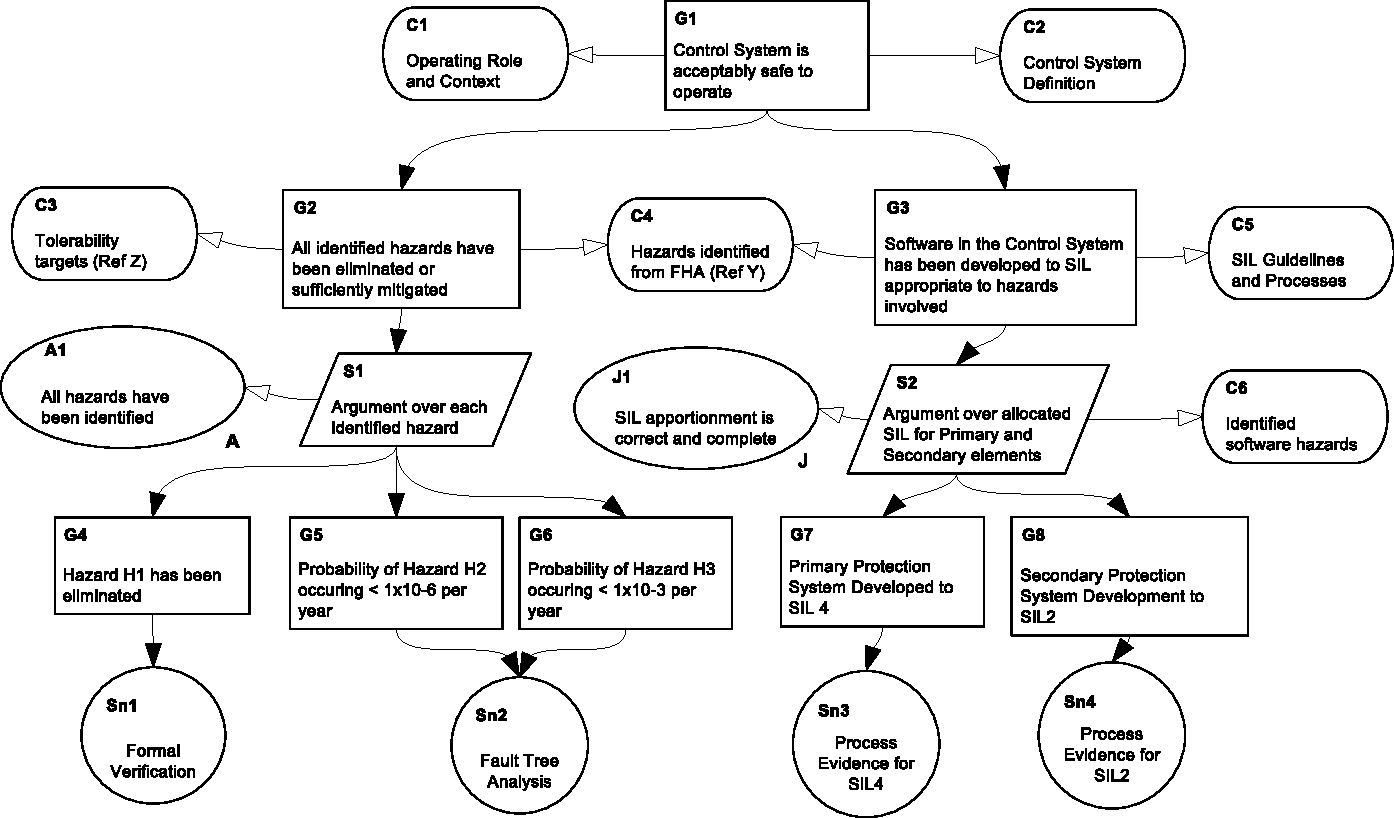
\includegraphics[width=\textwidth]{example_argument.pdf}
  \caption{An example GSN argument, about a safety case,
    from the GSN specification \cite{gsnstandard}}
  \label{fig:example}
\end{figure}




\section{Artoo}

Artoo (Argumentation Tool) is a web-based tool for drawing graph structures, specifically using the GSN syntax. It was developed by Paul Andrews at the York Computational Immunology Lab, and is therefore particularly well-suited to using the GSN to argue about biological simulations, \todo{how?} as \citet*{royal} do in a paper which both introduces Artoo and the use of the the argumentation (specifically the GSN) for this \ldots \todo{a bit clumsy?}

\ldots

Artoo is available for free under a GNU GPLv3 licence. Similar tools also exist for drawing GSN arguments, but they are largely commercial and 

\begin{figure}
  \centering
  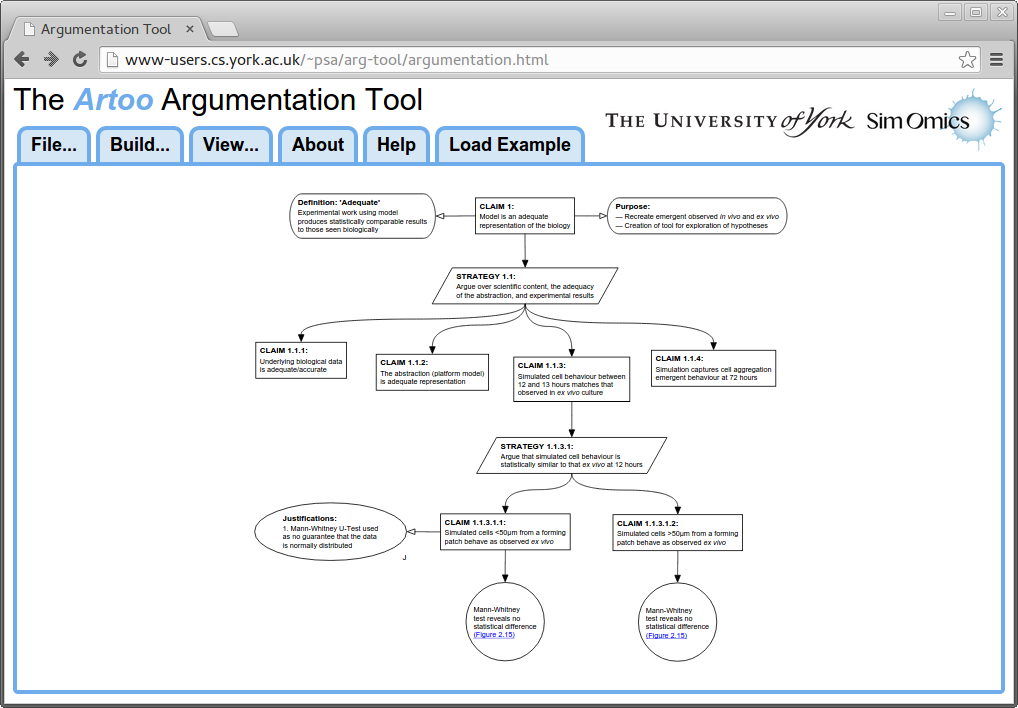
\includegraphics[width=\textwidth]{graphics/artoo_screenshot.png}
  \caption{The Artoo tool, displaying an argument }
\end{figure}




\section{Automatic layout of GSN arguments in the Artoo tool}

Currently, users 

This [report/project/thing] will \ldots

  \begin{enumerate}
    \item
      \begin{itemize}
      \item ,
    \end{itemize}
  \end{enumerate}

\subsection{Problem definition}

Typically, a graph layout algorithm takes as its inputs a set of nodes and a set of edges, [and outputs \ldots] [not a controversial statement but might cite].
In the case of a GSN argument, there is additional information associated with the input graph:

\begin{itemize}
  \item
    Nodes have sizes, rather than being simple points. \todo{not \emph{that} unusual, but \emph{a bit} unusual~ \ldots }
  \item
    There are multiple types of node and edge, and these should influence where a node is place. The GSN specification's layout guidance suggests that parent and child goals, stategies and solutios should be placed 
\end{itemize}

Artoo also allows the drawing of invalid GSN argments ...
if the graph layout [thing] is to be executed every time the graph is edited, then it must accept these .
If the algorithm [is exposed to the user by a] button, then there is the poissibility of checking 

Already, Artoo only works a limited set of web browsers: recent versions of \ldots
The features added in this project will not interact with the browser in any new way -- only needing to change the position of nodes, using functions already in the code -- it is very unlikely that there will be any problems \ldots